\begin{problem}[12.]
    $r = \frac{2}{1 + \sin(\theta)}$
\end{problem}

\begin{solution}
    Upon inspection we can pretty much solve this guy. $e=1$ which means we have a parabola. As such $d=2$ and our directrix is at $y=2$ based on our given theorem. Our focus is at $(0,0)$ which tells us our parabola is opening down AND the vertex must be at $(0,1)$. Lastly our focal diameter is the same as in problem 9, so $4$. \bigskip
    
    With this information I give the plot below. \bigskip
    
    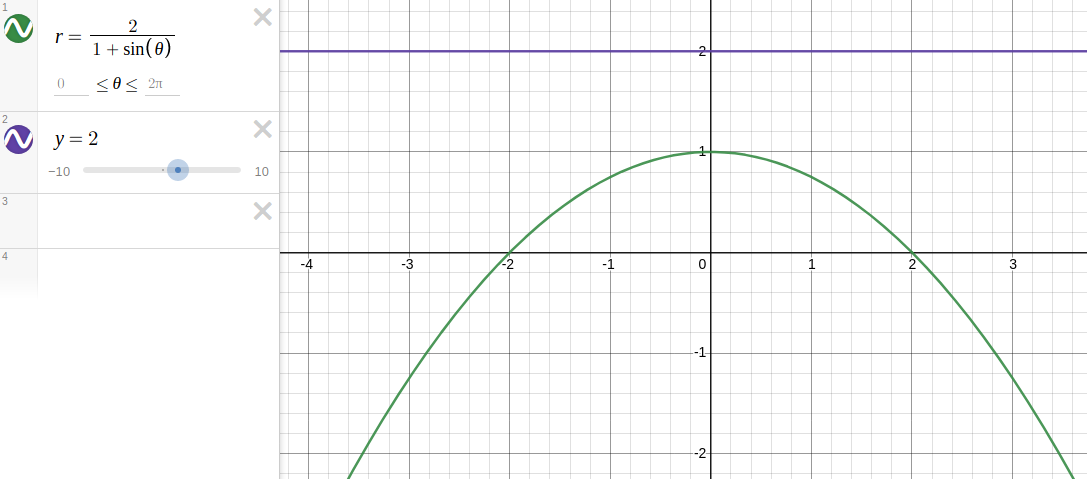
\includegraphics[scale=0.4]{images/pr_12.png}
\end{solution}